% This is text associated with the open textbook "Open Electromagnetics"
% See immediately below for author, date
% This work is licensed under the Creative Commons Attribution-ShareAlike 4.0 International License. (CC BY-SA 4.0) 
% To view a copy of the license, visit http://creativecommons.org/licenses/by-sa/4.0/

%ORB TITLE Charge and Electric Field for a Perfectly Conducting Region
%ORB AUTHOR 0        # S.W. Ellingson, Virginia Tech (ellingson@vt.edu)
%ORB DATE 20180806   # yyyymmdd
%ORB ABSTRACT Charge and Electric Field for a Perfectly Conducting Region

\label{m0025_Charge_and_Electric_Field_for_a_Perfectly_Conducting_Region} % <-- Must match name of this file and module directory name.  Don't mess with this!

In this section, we consider the behavior of charge and the electric field in the vicinity of a perfect electrical conductor (PEC).
\index{conductor!perfect}

First, note that the electric field -- both the electric field intensity {\bf E} and electric flux density {\bf D} -- throughout a PEC region is zero.
This is because the electrical potential throughout a PEC region must be constant.
(This idea is explored further in Section~\ref{m0010_Conductivity}.)
Recall that the electric field is proportional to the spatial rate of change of electrical potential (i.e., ${\bf E}=-\nabla V$; Section~\ref{m0063_Electric_Field_as_the_Gradient_of_Potential}).
Thus, the electric field must be zero throughout a PEC region.

Second, 
the electric field is oriented directly away from (i.e., perpendicular to) the PEC surface, and the magnitude of ${\bf D}$ is equal to the surface charge density $\rho_s$ (C/m$^2$) (Section~\ref{m0021_Boundary_Conditions_on_D}). 

Now we address the question of charge distribution; i.e., the location and density of charge.
Consider the scenario shown in Figure~\ref{m0025_fFlatSlab}.
%
\begin{figure}[b!]
\begin{center}
\pdftooltip{{  % note double braces
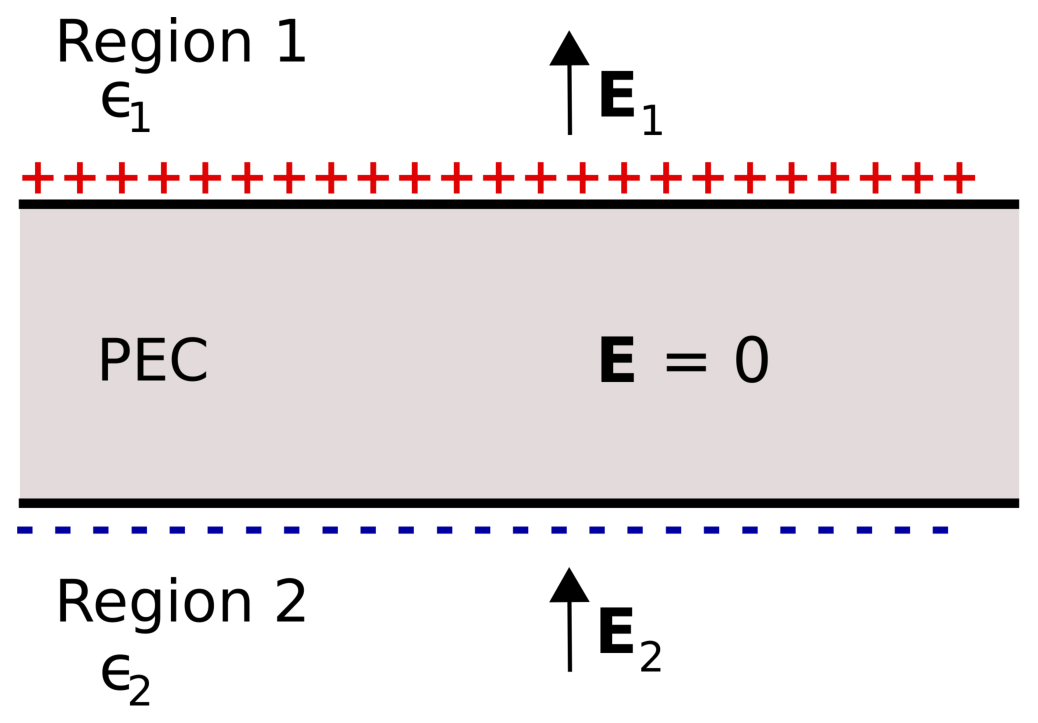
\includegraphics[width=2.5in]{modules/m0025_fFlatSlab.eps}
% https://commons.wikimedia.org/wiki/File:M0025_fFlatSlab.svg
}}{Region 1, above the slab, is shown as positively charged in field E sub 1, and Region 2, below the slab, is shown as negatively charged in E sub 2.}
\end{center} 
\centerline{\scriptsize 
\copyright~\hyperref[m0025_fFlatSlab_Credit]{K.\ Kikkeri}
\href{https://creativecommons.org/licenses/by-sa/4.0/}{CC BY~SA 4.0} 
} 
\caption{
\label{m0025_fFlatSlab}
An infinite flat slab of PEC in the presence of an applied electric field. 
}
\end{figure}
%
Here, a flat slab of PEC material is embedded in dielectric material.\footnote{For the purposes of this section, it suffices to interpret ``dielectric'' as a ``nonconducting and well characterized entirely in terms of its permittivity.''  For more, see Section~\ref{m0107_Dielectric_Media}.}
The thickness of the slab is finite, whereas the length and width of the slab is infinite.
The region above the slab is defined as Region~1 and has permittivity $\epsilon_1$.
The region below the slab is defined as Region~2 and has permittivity $\epsilon_2$.
Electric fields ${\bf E}_1$ and ${\bf E}_2$ are present in Regions~1 and 2, respectively, as shown in Figure~\ref{m0025_fFlatSlab}.
To begin, let us assume that these fields are the result of some external stimulus that results in the direction of these fields being generally upward, as shown in Figure~\ref{m0025_fFlatSlab}.

Now, what do we know about ${\bf E}_1$ and ${\bf E}_2$?
First, both fields must satisfy the relevant boundary conditions.
That is, the component of ${\bf E}_1$ that is tangent to the upper PEC surface is zero, so that ${\bf E}_1$ is directed entirely in a direction perpendicular to the surface.  
Similarly, the component of ${\bf E}_2$ that is tangent to the lower PEC surface is zero, so that ${\bf E}_2$ is directed entirely in a direction perpendicular to the surface. 
At this point we have not determined the magnitudes or signs of ${\bf E}_1$ and ${\bf E}_2$; we have established only that there are no non-zero components tangential to (i.e., parallel to) the PEC surfaces.

Next, recall that the electric field must be zero within the slab. 
This means that there must be zero net charge within the slab, since any other distribution of charge will result in a non-zero electric field, and subsequently a potential difference between locations within the slab. 
Therefore:
%
%ORB HIGHLIGHT
\begin{mdframed}[backgroundcolor=yellow!20,nobreak=true] 
There can be no static charge \emph{within} a PEC. 
\end{mdframed}
%
It follows that
%
%ORB HIGHLIGHT
\begin{mdframed}[backgroundcolor=yellow!20,nobreak=true] 
Charge associated with a PEC lies entirely on the surface. 
\end{mdframed}

Outside the slab, the boundary conditions on ${\bf D}_1$ and ${\bf D}_2$ in the dielectric regions require these fields to be non-zero when the surface charge density on the PEC is non-zero.
The surface charge supports the discontinuity in the normal component of the electric fields.
Specifically, ${\bf D}_1$ and ${\bf D}_2$ have the same magnitude $\left|\rho_s\right|$ because the surface charge densities on both sides of the slab have equal magnitude.
However, the electric field intensity ${\bf E}_1={\bf D}_1/\epsilon_1$, whereas ${\bf E}_2={\bf D}_2/\epsilon_2$; i.e., these are different.
That is, the electric field intensities are unequal unless the permittivities in each dielectric region are equal.

%%% ORIGINAL VERSION OF PARAGRAPH, USES SINGLE CUBE AS AN EXAMPLE %%%%%%%%%%%%%%%%%%%%%%%%% 
%% TODO: Maybe make this a problem?
% Finally, let us consider the effect if the length and width of the slab are reduced from infinity, forming a cube in which the length of each side is equal to the thickness of the original slab.  This is shown in Figure~\ref{m0025_fCube}.  For simplicity we have also set $\epsilon_1=\epsilon_2$, so the conductor is embedded in a single homogeneous material.  In this case the situation is as shown in Figure~\ref{m0025_fCube}.  Note that electric field lines now bend in the dielectric so as to satisfy the requirement that the tangential component of the electric field be zero on the surface of the cube.  Also note that the charge distribution arranges itself on the surface of the cube so as to maintain constant potential within the cube.
%
% \begin{figure}
% \begin{center}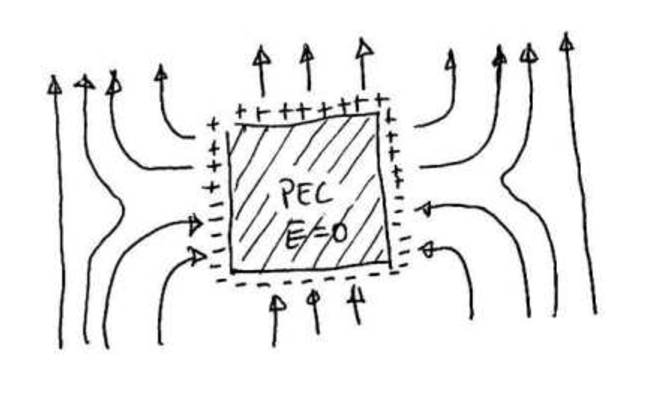
\includegraphics[width=2.5in]{modules/m0025_fCube.eps}\end{center} 
% %\vspace{2in}
% % ***WikipediaCommonsURL
% %\centerline{\scriptsize 
% %\copyright~\hyperref[***_Credit]{author} 
% %\href{https://creativecommons.org/licenses/by-sa/4.0/}{CC BY~SA 4.0} 
% %} 
% \caption{
% \label{m0025_fCube}
% A PEC cube in the presence of an applied electric field. 
% }
% \end{figure}

%%% NEW VERSION OF PARAGRAPH, USES FOUND FIGURE (POINT CHARGE AND MULTIPLE SHAPES) INSTEAD OF SINGLE CUBE %%%%%%%%%%%%%%%%%%%%%%%%% 
Finally, let us consider the structure of the electric field in more general cases.  
Figure~\ref{m0025_fPEC_field_lines} shows field lines in a homogeneous dielectric material in which a point charge and PEC regions of various shapes are embedded. 
Note that electric field lines now bend in the dielectric so as to satisfy the requirement that the tangential component of the electric field be zero on PEC surfaces.
Also note that the charge distribution arranges itself on the PEC surfaces so as to maintain zero electric field and constant potential within the cube.
%
\begin{figure}
\begin{center}
\pdftooltip{{  % note double braces
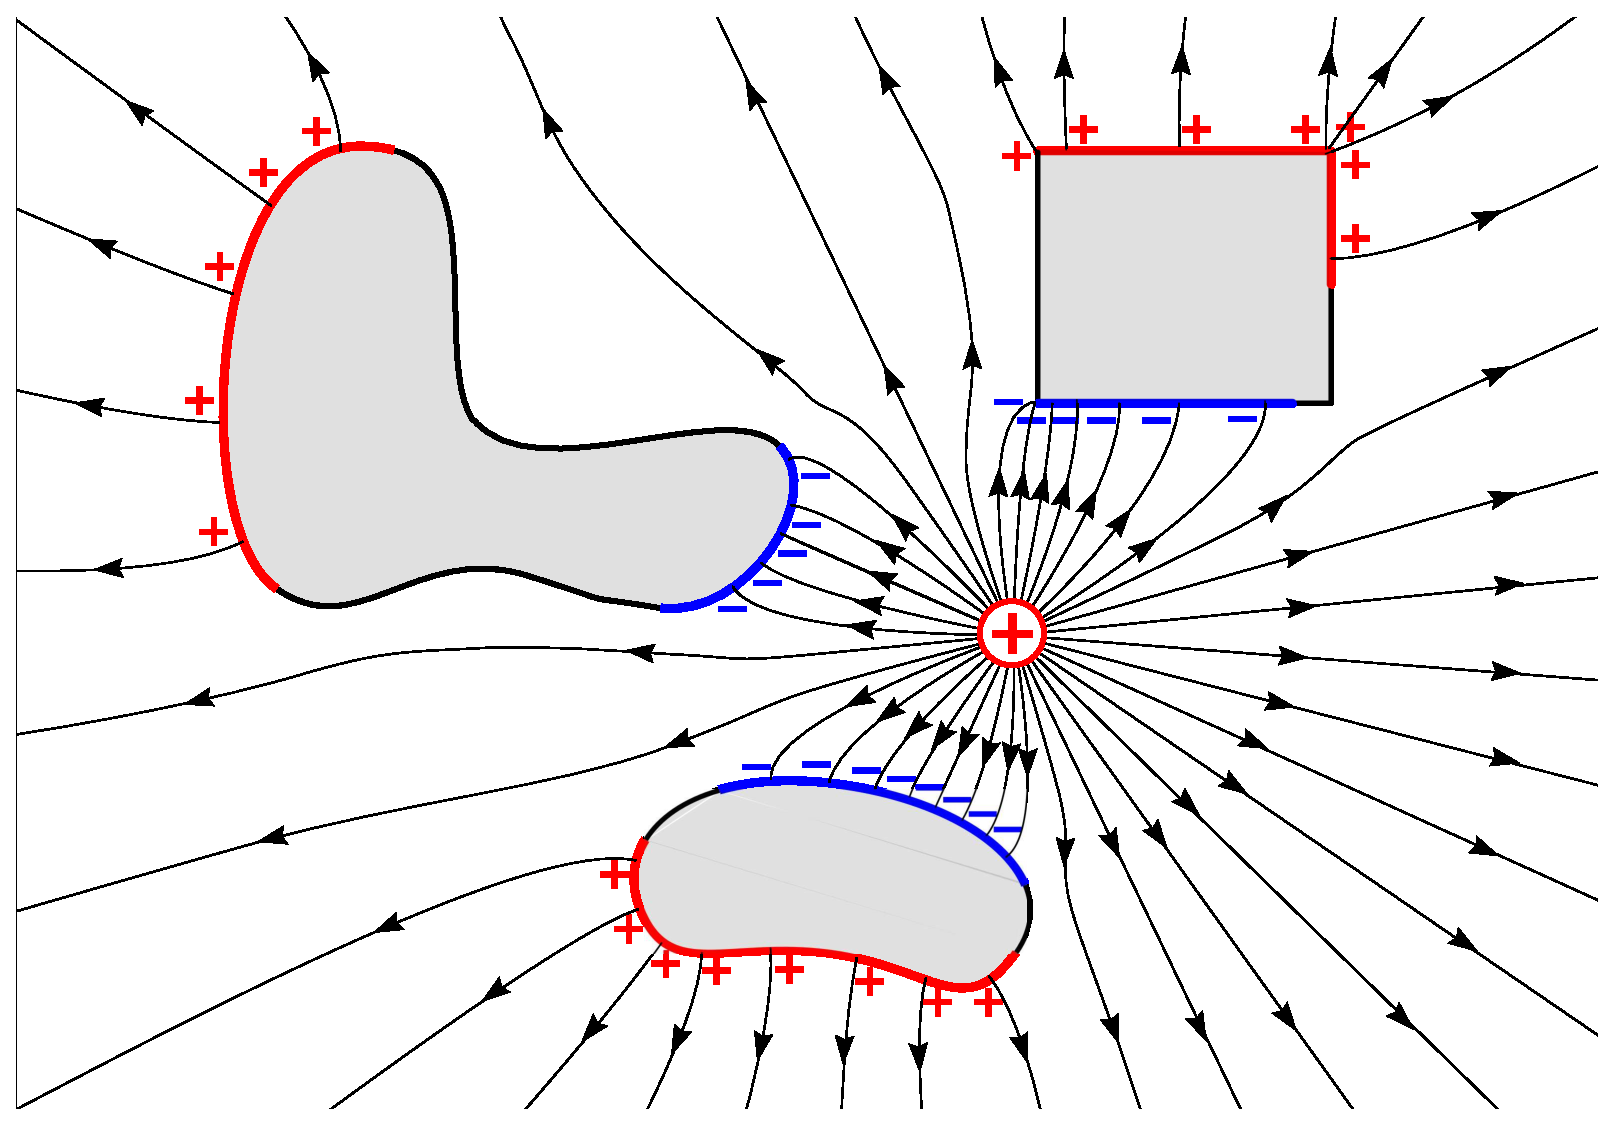
\includegraphics[width=\columnwidth]{modules/m0025_Electrostatic_induction_SE170813.eps}
% https://commons.wikimedia.org/wiki/File:Electrostatic_induction.svg
}}{A positive point charge is surrounded by three arbitrary, grey shaped PEC regions: one to the upper right, one to the directly below, and one to the upper left. From that particle extends electric field lines in all directions. Where the electric field lines meet the arbitrary regions the regions are labeled negative.}
\end{center} 
\centerline{\scriptsize 
by~\hyperref[m0025_fPEC_field_lines_Credit]{C.\ Burks} (modified) 
% public domain
} 
\caption{
\label{m0025_fPEC_field_lines}
Electric field lines due to a point charge in the vicinity of PEC regions (shaded) of various shapes. 
}
\end{figure}

